\documentclass[12pt]{handout}

\title{Dog on the beach}
\course{Math 1181H}
\author{Jim Fowler}
\date{September 2012} 

\usepackage{amsmath}
\usepackage{sagetex}
\usepackage{tikz}
\usetikzlibrary{decorations}
\usetikzlibrary{decorations.pathmorphing}
\usetikzlibrary{decorations.pathreplacing}
\usepackage{multicol}

\newcommand{\meters}{\mathrm{m}}
\newcommand{\seconds}{\mathrm{s}}

\begin{document}
\maketitle

Yesterday, we talked about the following problem.
\begin{multicols}{2}
\begin{quote}
  A beach runs perfectly east-west; a perfectly spherical dog is $5\,\meters$ north of the edge of the water, and a ball floats
  motionlessly $10\,\meters$ south and $10\,\meters$ east of the dog;
  the dog is somewhat injured, and runs at speed of $1\,\meters/\seconds$ on the sand, and swims at a speed of $s\,\meters/\seconds$.  Along what path should the dog travel to get to
  the ball as quickly as possible?
\end{quote}
\columnbreak
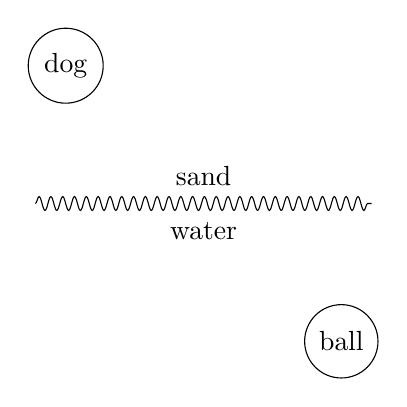
\begin{tikzpicture}[scale=0.35]
  \node[draw=black,circle] at (0,5) {dog};
\draw[decorate, decoration = {snake, segment length = .15cm}] (-1.1,0) -- (11.1,0);
  \node[draw=black,circle] at (10,-5) {ball};
  \node[yshift=10pt] at (5,0) {sand};
  \node[yshift=-10pt] at (5,0) {water};
\end{tikzpicture}
\end{multicols}

There are two ways of approaching this problem.

\subsection*{Via algebra and the Pythagorean theorem}

\begin{sagesilent}
s = var('s')
f = sqrt(5^2 + x^2) + (1/s) * sqrt(5^2 + (10-x)^2)
df = derivative(f,x)
\end{sagesilent}

\begin{multicols}{2}
  Suppose the dog enters the water $x\, \meters$ along the coastline.
  Then, by the Pythagorean theorem, the total travel time in seconds is
  \[
  f(x) = \sage{f}.
  \]
  Differentiating, we get
  \[
  f'(x) = \sage{df}.
  \]
  Now we look for a value of $x$ which makes $f'(x) = 0$.

\columnbreak

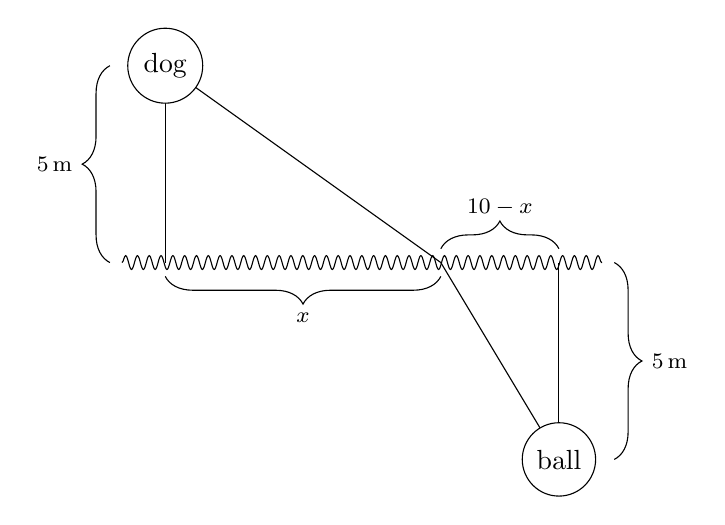
\begin{tikzpicture}[scale=0.5]
\draw[decorate, decoration = {snake, segment length = .15cm}] (-1.1,0) -- (11.1,0);
\draw (0,5) -- (0,0);
\draw (10,-5) -- (10,0);
\draw (0,5) -- (7,0);
\draw (7,0) -- (10,-5);
\draw [decorate,decoration={brace,amplitude=10pt,mirror},yshift=-10pt] (0,0) -- (7,0) node [black,midway,yshift=-15pt] {\footnotesize $x$};
\draw [decorate,decoration={brace,amplitude=10pt},yshift=10pt] (7,0) -- (10,0) node [black,midway,yshift=15pt] {\footnotesize $10-x$};

\draw [decorate,decoration={brace,amplitude=10pt,mirror},xshift=-40pt] (0,5) -- (0,0) node [black,midway,xshift=-20pt] {\footnotesize $5\,\meters$};
\draw [decorate,decoration={brace,amplitude=10pt},xshift=40pt] (10,0) -- (10,-5) node [black,midway,xshift=20pt] {\footnotesize $5\,\meters$};

  \node[draw=black,fill=white,circle] at (0,5) {dog};
  \node[draw=black,fill=white,circle] at (10,-5) {ball};
\end{tikzpicture}
\end{multicols}

\begin{sagesilent}
equation = (df == 0).subtract_from_both_sides(df.operands()[0])
\end{sagesilent}

To look for places where $f'(x) = 0$, we want
\[
\sage{equation}
\]
Since $0 \leq x \leq 10$, we can rewrite both sides as a square root,
co\[
\sage{sqrt(equation.lhs()^2) == sqrt(equation.rhs()^2)},
\]
and then take reciprocals to get
\[
\sage{sqrt(1/equation.lhs()^2) == sqrt(1/equation.rhs()^2)},
\]
and then simplify what is under the radicals, to get
\[
\sage{sqrt(s^2*(1/(s*equation.lhs())^2).partial_fraction()) ==  sqrt((1/equation.rhs()^2).partial_fraction())}.
\]
Squaring both sides,
\begin{sagesilent}
equation = (s^2*(1/(s*equation.lhs())^2).partial_fraction()) == ((1/equation.rhs()^2).partial_fraction())
\end{sagesilent}
\[
\sage{equation}.
\]
Now move everything to one side, producing
\begin{sagesilent}
equation = equation.rhs().expand() - equation.lhs().expand() == 0
\end{sagesilent}
\[
\sage{equation}.
\]
This I can then put over a common denominator, specifically
\[
\sage{equation.simplify_rational()},
\]
which vanishes provided the numerator (which we'll $p(x)$) does, that
is,
\begin{sagesilent}
  polynomial = equation.simplify_rational().lhs().numerator()
\end{sagesilent}
\[
p(x) = \sage{polynomial == 0}.
\]
We'll call the denominator $q(x) =
\sage{equation.simplify_rational().lhs().denominator()}$ and note that $q(x)$ factors as $\sage{factor(equation.simplify_rational().lhs().denominator())}$, so $q(x)$ is nonnegative when $0 \leq x \leq 10$.

Recall our goal is to find $x$ so that $f'(x) = 0$, and now it
suffices that $p(x) = 0$, but $p(x)$ is a \textit{quartic}, so, yes,
it is solvable, but no, it won't be easy to solve.  The quartic
formula is terrible!  If you think it will be easy, just try setting
$s = 2\, \meters/\seconds$.  In that case, the polynomial $p(x)$ is
\[
\sage{polynomial.substitute(s==2)}
\]
which does not factor into quadratics with rational coefficients.  Our
dog, even armed with a straightedge and compass, would have trouble
figuring out the best place to cross into the water.

There are some things we can say.  It's ``physically'' clear that this
polynomial $p(x)$ can only have one root in the interval $[0,10]$, so that
\begin{align*}
p(0) &= \sage{polynomial.substitute(x==0)} > 0, \\
p(5) &= \sage{polynomial.substitute(x==5)}, \mbox{ and } \\
p(10) &= \sage{polynomial.substitute(x==10)} < 0
\end{align*}
hold is qualitatively significant, in light of the intermediate value theorem; note that $p(5) < 0$ when $s > 1$ and $p(5) > 0$
when $s < 1$.  This reflects the fact that when $s > 1$, the dog can
swim faster than he can ``run,'' so the root to $p(x)$ must lie between $0$ and $5$.

\pagebreak

\subsection*{Via trigonometry}

Perhaps you did not find the previous algebraic solution very enlightening.  I don't blame you.  Remember we differentiated to get
\[
f'(x) = \sage{df}
\]
and now we will reinterpret this in terms of trigonometry.  Let's label a couple angles as $\theta$ and $\varphi$ as shown below.
\begin{center}

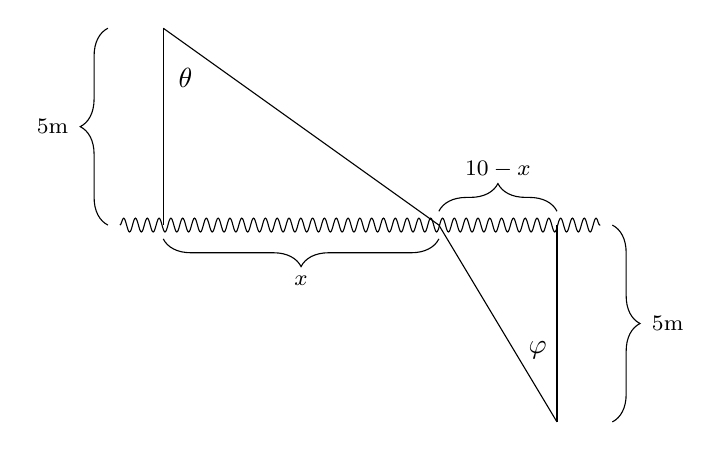
\begin{tikzpicture}[scale=0.5]
\draw[decorate, decoration = {snake, segment length = .15cm}] (-1.1,0) -- (11.1,0);
\draw (0,5) -- (0,0);
\draw (10,-5) -- (10,0);
\draw (0,5) -- (7,0);
\draw (7,0) -- (10,-5);
\draw [decorate,decoration={brace,amplitude=10pt,mirror},yshift=-10pt] (0,0) -- (7,0) node [black,midway,yshift=-15pt] {\footnotesize $x$};
\draw [decorate,decoration={brace,amplitude=10pt},yshift=10pt] (7,0) -- (10,0) node [black,midway,yshift=15pt] {\footnotesize $10-x$};

\draw [decorate,decoration={brace,amplitude=10pt,mirror},xshift=-40pt] (0,5) -- (0,0) node [black,midway,xshift=-20pt] {\footnotesize $5 \meters$};
\draw [decorate,decoration={brace,amplitude=10pt},xshift=40pt] (10,0) -- (10,-5) node [black,midway,xshift=20pt] {\footnotesize $5 \meters$};

\node[xshift=8pt,yshift=-18pt] at (0,5) {$\theta$};
\node[xshift=-7pt,yshift=26pt] at (10,-5) {$\varphi$};

\end{tikzpicture}
\end{center}
Then we can interpret the terms in $f'(x)$ via trigonometry.  The first term,
\[
\sage{df.operands()[0]},
\]
is $\sin \theta$.  The second term,
\[
\sage{df.operands()[1]},
\]
is $\displaystyle\frac{-1}{s} \cdot \sin \varphi$.  So we can write
\[
f'(x) = \sin \theta - \frac{1}{s} \sin \varphi.
\]
Now we are looking for an $x$ which makes $f'(x) = 0$, meaning we want
\[
s \cdot \sin \theta = \sin \varphi.
\]
At this point, we've stumbled upon \textit{Snell's law} describing
refraction, but we still don't have instructions to give to the dog.
There's a constraint we can express in terms of $\theta$ and
$\varphi$: since $x = 5 \tan \theta$ and $10 - x = 5 \tan \varphi$, we must have
\[
5 \tan \theta + 5 \tan \varphi = 10,
\]
So for the dog to know which way to run, it suffices to solve the system of equations
\begin{align*}
s \cdot \sin \theta &= \sin \varphi \\
\tan \theta &= 2 - \tan \varphi
\end{align*}
which, superficially, looks a lot nicer than the terrible polynomial $p(x)$ we encountered earlier.  But is it any better?

\subsection*{A concrete example}

Let's set $s = 2$.  In that case, the polynomial is 
\begin{align*}
  p(x) &= \sage{polynomial}  \\
       &= \sage{polynomial.substitute(s==2)}.
\end{align*}
We can try plugging in some values, such as
\begin{sagesilent}
  two = var('two',latex_name='\cdot 2')
  three = var('three',latex_name='\cdot 3')
\end{sagesilent}
\begin{align*}
  p(2) &= \sage{polynomial.substitute(s==2).substitute(x==two)} \\
       &= \sage{polynomial.substitute(s==2).substitute(x==2)} > 0\\
  p(3) &= \sage{polynomial.substitute(s==2).substitute(x==three)} < 0 \\
       &= \sage{polynomial.substitute(s==2).substitute(x==3)}
\end{align*}
\begin{sagesilent}
  root = find_root(polynomial.substitute(s==2),0,10)
  digit_count = 5
  under_root = n(floor(10^(digit_count-1) * root)/10^(digit_count-1),digits=digit_count)
  over_root = n(ceil(10^(digit_count-1) * root)/10^(digit_count-1),digits=digit_count)
\end{sagesilent}
and so the root lies between $2$ and $3$.  More work would reveal that
the root is between \sage{under_root} and \sage{over_root}, that is,
about $30/13$.  The actual value is
\begin{sagesilent}
  part = 125000/27*sqrt(3)*sqrt(173) + 3453125/27
  root = [z.rhs() for z in solve(polynomial.substitute(s==2)==0,x) if z.rhs() > 0][0]
  r = var('r')
  root = root.substitute_expression(part==r)
\end{sagesilent}
$$
\sage{root}
$$
where $r = (\sage{27*part})/27$.

Perhaps it is easier to solve the system of trigonometric equations?
We want to find a $\theta$ which satisfies
\begin{align*}
2 \cdot \sin \theta &= \sin \varphi \mbox{ and }\\
\tan \theta &= 2 - \tan \varphi
\end{align*}
for some $\varphi$.  One way to get a sense of this is to graph the points in the $(\theta,\varphi)$-plane which satisfy these equations.

\begin{sagesilent}
  p = plot([arcsin(2*sin(x)),arctan(2-tan(x))],-pi/2,pi/2)
\end{sagesilent}
\begin{center}
  \scalebox{0.7}{\sageplot{p}}
\end{center}

\pagebreak

\begin{sagesilent}
  manyplots = plot([arctan(2-tan(x))] + [arcsin(i*sin(x)/10) for i in range(1,50)],-pi/2,pi/2)
\end{sagesilent}
\begin{center}
  \sageplot{manyplots}
\end{center}

% arcsin(2*sin(x)),arctan(2-tan(x)

% or in other words, $\tan \varphi = 2 - \tan \theta$
% Since
% \[
% \sin \varphi = \frac{\tan \varphi}{\sqrt{\tan^2 \varphi + 1}}.
% \]
% we then have
% \[
% s \cdot \sin \theta = \frac{\tan \varphi}{\sqrt{\tan^2 \varphi + 1}} = \frac{2 - \tan \theta}{\sqrt{(2 - \tan \theta)^2 + 1}} =
% \frac{2 - \tan \theta}{\sqrt{5 + \tan^2 \theta - 4 \tan \theta}}
% \]
% which in terms of $\tan \theta$ alone is
% \[
% s \frac{\tan \theta}{\sqrt{\tan^2 \theta + 1}} = \frac{2 - \tan \theta}{\sqrt{5 + \tan^2 \theta - 4 \tan \theta}}
% \]

% we then have
% $$
% s \cdot \sin \theta = \sin \varphi \frac{\tan \varphi}{\sqrt{\tan^2 \varphi + 1}}
% $$

% Since $s \cdot \sin \theta = \sin \varphi$, we have
% $$
% \cos \varphi = \sqrt{1 - \sin^2 \varphi} = \sqrt{ 1 - s^2 \sin^2 \theta },
% $$
% so we can rewrite $5 \tan \varphi$ as 
% $$
% 5 \tan \varphi
% = 5 \frac{s \cdot \sin \theta}{\sqrt{ 1 - s^2 \sin^2 \theta }}
% = 5 \sqrt{\frac{s^2 \cdot \sin^2 \theta}{ 1 - s^2 \sin^2 \theta }}
% $$
% All this means that the condition on $\theta$ is given by
% $$
% 5 \tan \theta + 5 \sqrt{\frac{s^2 \cdot \sin^2 \theta}{ 1 - s^2 \sin^2 \theta }} = 10
% $$
% We rearrange a bit to get
% $$
% \sqrt{\frac{s^2 \cdot \sin^2 \theta}{ 1 - s^2 \sin^2 \theta }} = 2 - \tan \theta
% $$
% and then square both sides to get
% $$
% \frac{s^2 \cdot \sin^2 \theta}{ 1 - s^2 \sin^2 \theta } = 4 + \tan^2 \theta - 4 \tan \theta.
% $$
% Multiplying both sides by $1 - s^2 \sin^2 \theta$ gives
% \begin{align*}
% s^2 \sin^2 \theta &= \left( 4 + \tan^2 \theta - 4 \tan \theta \right) \left( 1 - s^2 \sin^2 \theta \right) \\
% \end{align*}


% BAD
% $$
% 1 = 5 s^2 \sin^2 \theta  + s^2 \cos^2 \theta - 4 s^2 \sin \theta \cos \theta.
% $$
% Using the identity $\sin^2 \theta + \cos^2 \theta = 1$ gives
% $$
% 1 = 4 s^2 \sin^2 \theta + s^2 - 4 s^2 \sin \theta \cos \theta,
% $$
% and collecting the $\theta$'s all on one side produces
% $$
% \frac{1 - s^2}{4s^2}  = \sin^2 \theta - \sin \theta \cos \theta.
% $$
% Now $\sin^2 \theta = \frac{1}{2} \left( 1 - \cos (2\theta) \right)$ and $\sin \theta \cos \theta = \frac{1}{2} \sin (2\theta)$, so we have
% $$
% \frac{1 - s^2}{2s^2}  =  1 - \cos (2\theta) - \sin (2\theta)
% $$
% which means we are looking for $\theta$ so that
% $$
% \sin (2\theta) + \cos(2 \theta) = \frac{3s^2 - 1}{2s^2}
% $$

% which means
% \[
% \tan \varphi = \frac{\tan \theta}{2\,\tan \theta - 1}.
% \]
% Since $\sin \varphi > 0$, we also have the trigonometric identity

% So the condition that $f'(x) = 0$ implies
% \begin{sagesilent}
% theta = var('theta')
% equation = s * sin(theta) == (tan(theta)/(2*tan(theta) - 1)) / sqrt( (tan(theta)/(2*tan(theta) - 1))^2 + 1 )
% \end{sagesilent}
% \[
% s \cdot \sin \theta = \sin \varphi = \frac{\frac{\tan \theta}{2\,\tan \theta - 1}}{\sqrt{\left( \frac{\tan \theta}{2\,\tan \theta - 1} \right)^2 + 1}} = \sage{equation.rhs()}
% \]
% We can replace tangent by sine over cosine to get
% \begin{sagesilent}
%   equation = equation.substitute(tan(theta)==sin(theta)/cos(theta))
% \end{sagesilent}
% \[
% \sage{equation}
% \]
% which simplifies to
% \begin{sagesilent}
%   equation = equation.full_simplify()
% \end{sagesilent}
% \[
% \sage{equation}
% \]

% \subsection*{Putting them together}

\end{document}

%%% Local Variables: 
%%% mode: latex
%%% TeX-master: t
%%% End: 
